%\textbf{Knowledge Graphs(KGs).} 
In this paper, a knowledge graph~\cite{Pan2016} is represented in a standard format for graph-structured data such as RDF. A   \vicf{\emph{knowledge graph}} $\mathcal{G}$  is a tuple $(\mathcal{E},\mathcal{R}, \mathcal{C},\mathcal{T} )$, where  $\mathcal{E}$ is a set of entities,  $\mathcal{R}$ is a set of relation types, $\mathcal{C}$ is a set of entity types,  and  $\mathcal{T}$ is a set of triples.
%Given a set of entities $\mathcal{E}$, relations $\mathcal{R}$, and triples $\mathcal{T}$, a knowledge graph $\mathcal{G}$ = ($\mathcal{E}$,$\mathcal{R}$,$\mathcal{T}$) is a set of tuples. 
Triples in $\mathcal{T}$ are 
%of the form  ($h,r,t$), 
either relation assertions $(h,r,t)$,
where $h,t \in \mathcal{E}$  are respectively the \emph{head} and \emph{tail} entities of the triple, and $r \in \mathcal{R}$ is the \emph{edge}  of the triple connecting  head and tail, or entity type assertions ($e$, $type$, $c$), where $e \in \mathcal{E}$ is an entity, $c\in \mathcal{C}$ is an entity type  and $type$ is  the instance-of relation~\cite{DBLP:series/ihis/Pan09}. %Equivalently, one can see  $\mathcal G$ as a First-order Logic (FOL) knowledge base with each triple  $(h,r,t) \in \mathcal G$ representing an atomic formula $r(h,t)$, with $r$ a binary relation name. In short, we consider schema-less KGs here.

\vic{We consider FOL queries that  use  existential quantification ($\exists$), conjunction ($\wedge$), disjunction ($\vee$) and negation ($\neg$) operations. We will work with FOL queries in Disjunctive Normal Form, i.e. represented as a disjunction of conjunctions. To introduce FOL queries, we assume that $\mathcal V_a \subset \mathcal E$ represents a set of  non-variable \emph{input anchor entities}, $V_1, \ldots, V_m$ denote \emph{existentially quantified variables} %\nb{Zhiwei: change to \emph{existentially quantified variable entities?}} 
and $V_?$ is the \emph{target variable}. %\nb{Zhiwei: change to \emph{target entities?}}.
%
A FOL query $\mathcal Q$  is a formula of the following form: }
%a Boolean function between head and tail entity. The function $r_{h\rightarrow t}$($\cdot$,$\cdot$) : $\mathcal{E}$ $\times$ $\mathcal{E}$ $\mapsto$ $\{$True, False$\}$, indicates whether the relation $r_{h\rightarrow t}$ between a pair of entities, i.e., ($e_{h}$, $e_{t}$), holds or not. Without loss of generality, for all triples ($e_{h}$,$r_{h\rightarrow t}$,$e_{t}$) in KGs, we have $r_{h\rightarrow t}$($e_{h}$,$e_{t}$) = True, i.e., the relation exist.
%
% \textbf{First-Order Logic (FOL).} FOL queries involve the logical operations using existential quantification ($\exists$), conjunction ($\wedge$), disjunction($\vee$), and negation($\neg$). Any FOL queries can be transformed into the equivalent Disjunctive Normal Form (DNF)~\cite{davey2002introduction}, which represents FOL queries as a disjunction of conjunctions. A FOL query $\mathcal{Q}$ in the dsjunctive normal form can be defined as: %the following form:
%\begin{equation*}
\begin{align*}
\mathcal{Q}[V_{?}] = & \,\, V_{?}\, . \, \exists V_{1}, \ldots, V_{m} : c_{1} \vee c_{2} \vee \ldots  \vee c_{n} 
% \text{ where }& \,\, c_{i} = e_{i1} \wedge \ldots \wedge e_{ik}, k \leq m \\
% &\text{ with   each} e_{ij} \text{is of one of the forms }
\end{align*}
%\end{equation*}
 %
\vic{ where  $c_{i} = e_{i1} \wedge \ldots \wedge$ $e_{ik}$, \emph{k} $\leq$ \emph{m} such that each $e_{ij}$ is of one of the following forms: $r(V_{a}, V)$, $\neg r(V_{a}, V)$,   $r(V_, V')$ or $\neg r(V, V')$, with $V_a \in \mathcal V_a$, $V \in \{V_{?}, V_{1},\ldots , V_{m}\}$, $V' \in \{V_{1},\ldots , V_{m}\}$,
   %\text{ with }  V_{i}, V_{j}\in \{V_{?}, V_{1}, ... , V_{m}\},
   $V \neq V'.$}%\nb{V: fixed was a leftover from previous notation}

 %
%$e_{ij}$ = 
%$r_{h\rightarrow t}$($e_{a}$, $e_{j}$) or $\neg$$r_{h\rightarrow t}$($e_{a}$, $e_{j}$) with $e_{j}$ $\in$ \{$e_{?}$, $e_{1}$, ... , $e_{m}$\}, 
%\par or $e_{ij}$ = $r_{h\rightarrow t}$($e_{i}$, $e_{j}$) or $\neg$$r_{h\rightarrow t}$($e_{i}$, $e_{j}$) with $e_{i}$, $e_{j}$ $\in$ \{$e_{?}$, $e_{1}$, ... , $e_{m}$\}, $e_{i}$ $\neq$ $e_{j}$. \\
%The variable $e_{?}$ is the \textit{target entity}, $e_{1}$ , ... , $e_{m}$ are existentially quantified bound entities, and $e_{a}$ $\in$ $\mathcal{E}$ represents the \textit{non-variable anchor entities}. 
\vic{The \emph{dependency graph (DG) of a query $\mathcal Q$} is a graphical representation of  $\mathcal Q$, where nodes correspond to variable or non-variable arguments in $\mathcal Q$ and edges correspond to relations in $\mathcal Q$.  Figure~\ref{fig_1} shows an example of a DG.}

\vic{We are interested in the multi-hop reasoning problem of answering  queries $\mathcal Q$ on KGs, which aims to find a set of entities $\llbracket \mathcal{Q}\rrbracket \subseteq \mathcal E$ such that\ $a \in \llbracket \mathcal{Q}\rrbracket $ iff $\mathcal Q[a]$ holds true.} %We refer to $\llbracket \mathcal{Q}\rrbracket$ as the \emph{answer set} of $\mathcal Q$.}

%\nb{Zhiwei: In my opinion, there is a gap between this paragraph and the previous paragraph, and I feel that the connection is not very close.}
%As an example of a dependency graph see the light gray shaded part in the Figure~\ref{fig_1}.}
%The \emph{dependency graph} corresponding to the certain $\mathcal Q$ can be shown in the light gray shaded part in the Figure~\ref{fig_1}.
%Given the logical query $\mathcal{Q}$ over KGs, answering the query is essentially finding the set of entities to satisfy $\llbracket$$\mathcal{Q}$$\rrbracket$ $\subseteq$ $\mathcal{E}$ where \emph{e} $\in$ $\llbracket$$\mathcal{Q}$$\rrbracket$ iff $\mathcal{Q}$[\emph{e}] = True. \\

% \textbf{Query Structure (QS).} The QS includes three types of nodes, namely \textit{anchor nodes}, \textit{variable nodes}, and \textit{target nodes}, and four logic operations, namely projection, intersection, disjunction, and negation, as shown in Figure \ref{fig_2}. We subdivide the QS into existential variable QS (EV-QS, grey nodes) and non-existential variable QS (NV-QS), according to whether the QS contains \textit{variable nodes}. 

% \begin{figure}[ht]
%     \centering
%     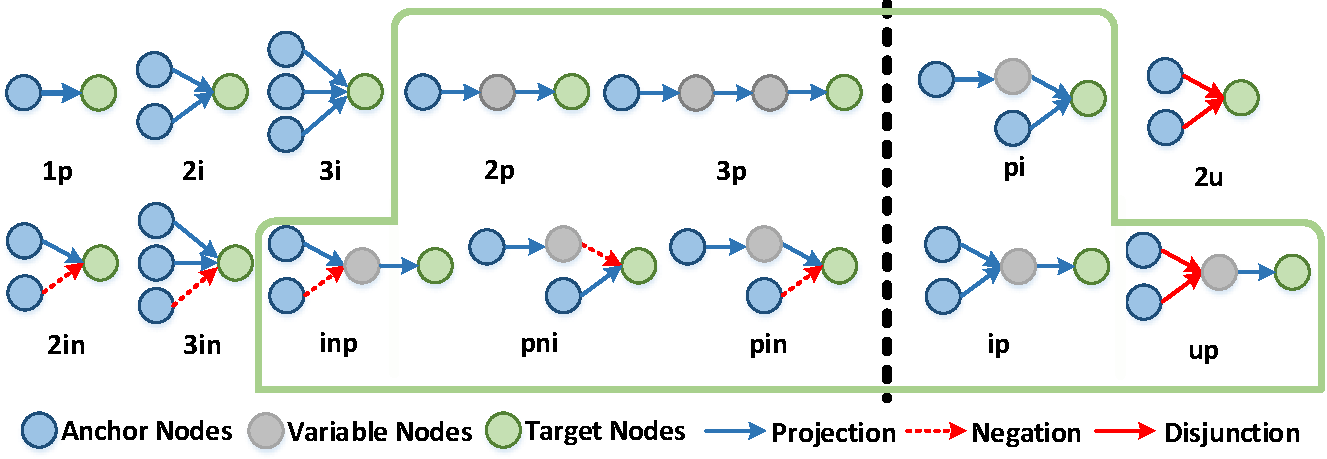
\includegraphics[width=0.5\textwidth]{img/query_pattern.pdf}
%     \caption{\textbf{Fourteen queries considered in the experiments.} Where `p', `i', `u', and `n' stand for `projection', `intersection', `union', and `negation', respectively. The numbers 1, 2, 3 indicate the number of relations. The left part divided by the black vertical dotted line is used in the training phase. Both queries are used in the validation and test phases. The solid green area represents the \emph{existential variable QS (EV-QS)}, while the remaining area denotes the \emph{non-existential variable QS (NV-QS)}. The differences between two areas lie in whether there exist variable nodes in the query sequence.}
%     \label{fig_2}
% \end{figure}